\documentclass[12pt]{article}
\usepackage[margin=2cm]{geometry}
\usepackage{amsmath}
\usepackage{graphicx}

\begin{document}

\noindent
The following table is from Particle Data Group.\footnote{\tt https://pdg.lbl.gov/2020/listings/rpp2020-list-muon.pdf}

\begin{center}
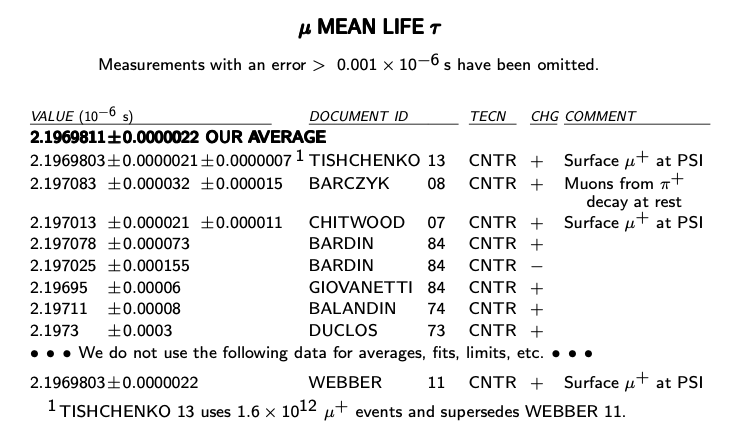
\includegraphics[scale=0.5]{muon-mean-life.png}
\end{center}

\noindent
From ``V minus A'' theory we have the following formula for muon lifetime $\tau$.
\begin{equation*}
\tau=\frac{96\pi^2h}{G_F^2\left(m_\mu c^2\right)^5}
\end{equation*}

\noindent
Symbol $G_F$ is Fermi coupling constant, $m_\mu$ is muon mass.

\bigskip
\noindent
From NIST\footnote{\tt https://physics.nist.gov/cuu/Constants/index.html} we have
\begin{align*}
G_F&=1.1663787\times10^{-5}\;\text{GeV}^{-2}
\\
m_\mu&=1.883531627\times10^{-28}\;\text{kilogram}
\\
h&=6.62607015\times10^{-34}\;\text{joule}\;\text{second}\;\text{(exact)}
\\
c&=299792458\;\text{meter}\;\text{second}^{-1}\;\text{(exact)}
\\
1\,\text{eV}&=1.602176634\times10^{-19}\;\text{joule}\;\text{(exact)}
\end{align*}

\noindent
Hence
\begin{equation*}
\tau=2.18735\times10^{-6}\,\text{second}
\end{equation*}

\noindent
The result is a bit smaller than the PDG value.
\begin{equation*}
\frac{\tau}{2.1969811\times10^{-6}\;\text{second}}=0.9956
\end{equation*}

\noindent
A muon decays into a muon neutrino, an electron anti-neutrino,
and an electron.
\begin{center}
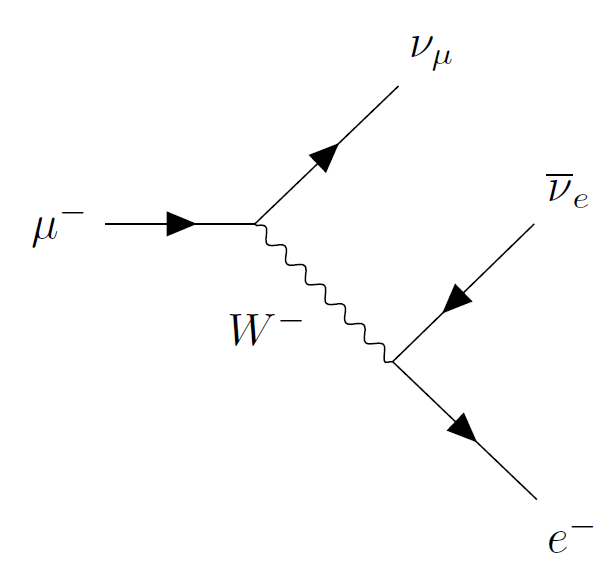
\includegraphics[scale=0.25]{muon-decay-diagram.png}
\end{center}

\begin{center}
\begin{tabular}{lllll}
Particle & Symbol & Momentum & Spinor (up) & Spinor (down)
\\[2ex]
Muon & $\mu^-$ & $p_1$ & $u_{11}$ & $u_{12}$
\\
Muon neutrino & $\nu_\mu$ & $p_2$ & $u_{21}$ & $u_{22}$
\\
Electron anti-neutrino & $\bar{\nu}_e$ & $p_3$ & $v_{31}$ & $v_{32}$
\\
Electron & $e^-$ & $p_4$ & $u_{41}$ & $u_{42}$
\end{tabular}
\end{center}

\noindent
We will use the following momentum vectors.
\begin{equation*}
p_1=
\underset{\substack{\\[1ex] \mu^-}}
{\begin{pmatrix}E_1\\p_{1x}\\p_{1y}\\p_{1z}\end{pmatrix}}
\qquad
p_2=
\underset{\substack{\\[1ex] \nu_\mu}}
{\begin{pmatrix}E_2\\p_{2x}\\p_{2y}\\p_{2z}\end{pmatrix}}
\qquad
p_3=
\underset{\substack{\\[1ex] \bar{\nu}_e}}
{\begin{pmatrix}E_3\\p_{3x}\\p_{3y}\\p_{3z}\end{pmatrix}}
\qquad
p_4=
\underset{\substack{\\[1ex] e^-}}
{\begin{pmatrix}E_4\\p_{4x}\\p_{4y}\\p_{4z}\end{pmatrix}}
\end{equation*}

\noindent
And we will also use the following Dirac spinors.
\begin{align*}
u_{11}&=\begin{pmatrix}E_1+m_1\\0\\p_{1z}\\p_{1x}+ip_{1y}\end{pmatrix}
&
u_{21}&=\begin{pmatrix}E_2+m_2\\0\\p_{2z}\\p_{2x}+ip_{2y}\end{pmatrix}
&
v_{31}&=\begin{pmatrix}p_{3z}\\p_{3x}+ip_{3y}\\E_3+m_3\\0\end{pmatrix}
&
u_{41}&=\begin{pmatrix}E_4+m_4\\0\\p_{4z}\\p_{4x}+ip_{4y}\end{pmatrix}
\\[2ex]
u_{12}&=
\underset{\substack{\\[1ex] \mu^-}}
{\begin{pmatrix}0\\E_1+m_1\\p_{1x}-ip_{1y}\\-p_{1z}\end{pmatrix}}
&
u_{22}&=
\underset{\substack{\\[1ex] \nu_\mu}}
{\begin{pmatrix}0\\E_2+m_2\\p_{2x}-ip_{2y}\\-p_{2z}\end{pmatrix}}
&
v_{32}&=
\underset{\substack{\\[1ex] \bar{\nu}_e}}
{\begin{pmatrix}p_{3x}-ip_{3y}\\-p_{3z}\\0\\E_3+m_3\end{pmatrix}}
&
u_{42}&=
\underset{\substack{\\[1ex] e^-}}
{\begin{pmatrix}0\\E_4+m_4\\p_{4x}-ip_{4y}\\-p_{4z}\end{pmatrix}}
\end{align*}

\noindent
The energy terms are total energy.
\begin{align*}
E_1&=\sqrt{(p_{1x})^2+(p_{1y})^2+(p_{1z})^2+m_1^2}
\\[1ex]
E_2&=\sqrt{(p_{2x})^2+(p_{2y})^2+(p_{2z})^2+m_2^2}
\\[1ex]
E_3&=\sqrt{(p_{3x})^2+(p_{3y})^2+(p_{3z})^2+m_3^2}
\\[1ex]
E_4&=\sqrt{(p_{4x})^2+(p_{4y})^2+(p_{4z})^2+m_4^2}
\end{align*}

\noindent
From the Feynman diagram above we have the following amplitude $\mathcal{M}_{abcd}$
where each letter in $abcd$ can be either 1 (spin up) or 2 (spin down).
\begin{equation*}
\mathcal{M}_{abcd}=\frac{G_F}{\sqrt{N}}
\left(\bar{u}_{4d}\gamma^\mu(1-\gamma^5)v_{3c}\right)
\left(\bar{u}_{2b}\gamma_\mu(1-\gamma^5)u_{1a}\right)
\end{equation*}

\noindent
Symbol $N$ is the following normalization constant.
\begin{equation*}
N=(E_1+m_1)(E_2+m_2)(E_3+m_3)(E_4+m_4)
\end{equation*}

\noindent
Recall that the magnitude squared of an amplitude is a probability density and also an observable.
\begin{equation*}
|\mathcal{M}_{abcd}|^2=\mathcal{M}_{abcd}^*\mathcal{M}_{abcd}
\end{equation*}

\noindent
In a typical muon decay experiment the spins are not observed.
Consequently, the experimental result is an average of spin states.
The average is computed by summing over all spin states and dividing by the number of inbound spin states,
in this case four.
(In the Feynman diagram, two particles have arrows pointing into vertices,
these are the inbound particles.
There are two spin states for $\mu^-$ and two spin states for $\bar{\nu}_e$.
Hence there are $2\times2=4$ inbound spin states.)
\begin{equation*}
\langle|\mathcal{M}|^2\rangle=
\frac{1}{4}
\sum_{a=1}^2\sum_{b=1}^2\sum_{c=1}^2\sum_{d=1}^2
|\mathcal{M}_{abcd}|^2
\end{equation*}

\noindent
The result is a simple formula.
\begin{equation*}
\langle|\mathcal{M}|^2\rangle=64G_F^2(p_1\cdot p_3)(p_2\cdot p_4)
\tag{1}
\end{equation*}

\noindent
In component notation we have
\begin{equation*}
\langle|\mathcal{M}|^2\rangle=64G_F^2
\bigg((p_1)^\alpha \; g_{\alpha\beta}\; (p_3)^\beta\bigg)
\bigg((p_2)^\gamma \; g_{\gamma\delta} \; (p_4)^\delta\bigg)
\end{equation*}
where
\begin{equation*}
g_{\mu\nu}=\begin{pmatrix}
1 & 0 & 0 & 0\\
0 & -1 & 0 & 0\\
0 & 0 & -1 & 0\\
0 & 0 & 0 & -1
\end{pmatrix}
\end{equation*}

\noindent
Muon decay rate $\Gamma$ is an average over all possible momenta.
(The simplified measure $dp$ represents a lengthy product of terms.)
\begin{equation*}
\Gamma=
\underset{\text{12 integrals}}
{\int\cdots\int}
\langle|\mathcal{M}|^2\rangle\,dp
\end{equation*}

\noindent
It can be shown that
\begin{equation*}
\Gamma=\frac{G_F^2 m_\mu^5}{192\pi^3}
\end{equation*}
where $m_\mu=m_1$.
Muon lifetime $\tau$ is the inverse of decay rate.
\begin{equation*}
\tau=\frac{192\pi^3}{G_F^2 m_\mu^5}
\end{equation*}

\noindent
In physical units for $c$ and $h$ we have
\begin{equation*}
\tau=\frac{96\pi^2h}{G_F^2\left(m_\mu c^2\right)^5}
\end{equation*}

\end{document}
